
\section{DDPG}\label{DDPGsection}

\subsection{Вывод из Deep Q-learning}

Схема DQN \ref{DQNalgorithm} имела принципиальный недостаток: мы не могли работать с непрерывными пространствами действий в силу необходимости постоянно считать операторы максимума и аргмаксимума
$$\max_a Q_{\theta}(s, a)$$
как для жадного выбора действия, так и для построения таргета в задаче регрессии. 

\needspace{7\baselineskip}
\begin{wrapfigure}{r}{0.35\textwidth}
\vspace{-0.3cm}
\centering
\includegraphics[width=0.3\textwidth]{Images/Qnetwork1.png}
\vspace{-0.3cm}
\end{wrapfigure}

Единственная возможная архитектура модели --- приём действий на вход вместе с состояниями, тогда поиск аргмаксимума проводить, в целом, можно, но дорого: инициализируем $a^0$ случайно, и устраиваем градиентный подъём по входу в модель:
$$a^{k+1} = a^k + \alpha \left. \nabla_a Q_{\theta}(s, a) \right|_{a = a^k}$$

Понятно, что такую процедуру устраивать по несколько раз за шаг дороговато. Однако, в глубинном обучении для таких проблем есть мега-универсальное решение: давайте задачу поиска аргмаксимума тоже аппроксимируем другой нейросетью! Максимум тогда можно будет считать, просто подставив в $Q_{\theta}$ вместо действия приближение этого аргмаксимума.

Итак, пусть $\pi_{\omega}(s)$ принимает на вход состояние $s$ и выдаёт аргмаксимум текущей аппроксимации Q-функции, то есть будем добиваться $\pi_{\omega}(s) \HM\approx \argmax\limits_a Q_{\theta}(s, a)$. Понятно, как обучать такую сеть:
$$Q_\theta(s, \pi_{\omega}(s)) \to \max_{\omega}$$

Весь алгоритм DQN оставляем неизменным с единственной модификацией, что на каждом батче также нужно сделать шаг оптимизации $\omega$. При этом каждый раз, когда в схеме необходимо считать максимум или аргмаксимум $Q_\theta$, используется $\pi_{\omega}(s)$.

В стандартном алгоритме DQN нам было необходимо считать $\max\limits_{a'} Q_{\theta^{-}}(s', a')$, и в дефолтной версии алгоритма использовалась таргет-сеть. Технически это означает, что для таргет-сети $Q_{\theta^{-}}(s', a')$ нам тоже нужно знать аргмаксимум, поэтому можно хранить старую версию вспомогательной функции $\pi_{\omega^{-}}(s)$. 

\begin{remark}
Считается, что это не так принципиально, поскольку использование <<свежей>> $\pi_{\omega}(s)$ при подсчёте таргета соответствует моделированию Double оценки (см. раздел \ref{subsec:doubledqn}). Все остальные модификации DQN также применимы.
\end{remark}

Итого мы получили, что для жадного выбора действия используется $\pi_{\omega}(s)$ (отсюда такое обозначение этой <<вспомогательной>> функции --- это фактически стратегия); а таргет для перехода $\T \coloneqq (s, a, r, s')$ вычисляется по формуле
$$y(\T) \coloneqq r + \gamma Q_{\theta^{-}}(s', \argmax_{a'} Q_{\theta^{-}}(s', a')) \approx r + \gamma Q_{\theta^{-}}(s', \pi_{\omega^{-}}(s))$$

Такой алгоритм называется Deep Deterministic Policy Gradient (DDPG), и название может сбить с толку: а причём здесь policy gradient?

\subsection{Вывод из Policy Gradient}

% В Policy Gradient подходе мы могли работать с непрерывными пространствами действий, например, выдавая стратегией $\pi$ среднее и диагональную матрицу ковариации из нормального распределения:
% $$\pi_\theta(a \mid s) = \N\left( \mu(s, \theta), \sigma^2(s, \theta)I \right)$$

В Policy Gradient алгоритмах мы получили формулу градиента нашего функционала, <<релаксировав>> задачу и перейдя к оптимизации в пространстве стохастических стратегий. Если пространство действий непрерывно, то такая релаксация на самом деле не обязательна. Предположим\footnote{даже если это не так, в будущем мы всё равно будем приближать эти Q-функции нейросетями, для которых всегда справедлива дифференцируемость по входу.} дифференцируемость любых Q-функций $Q^{\pi}(s, a)$ по действиям $a$. Попробуем посчитать градиент по параметрам стратегии в случае детерминированной стратегии $\pi_\theta(s)$:

\begin{theoremBox}[label=th:dpg]{Deterministic Policy Gradient} В непрерывных пространствах действий в предположении дифференцируемости Q-функций по действиям:
\begin{equation}\label{dpg}
\nabla_\theta J(\pi_\theta) = \frac{1}{1 - \gamma}\E_{d_{\pi_\theta}(s)} \nabla_\theta \pi_\theta(s) \left. \nabla_a Q^{\pi}(s, a) \right|_{a = \pi_\theta(s)}
\end{equation}
\beginproof
$$\nabla_\theta V^{\pi_\theta}(s) = \{\text{VQ уравнение \eqref{VQ}}\} = \nabla_\theta \E_{a \sim \pi_\theta(s)} Q^{\pi_\theta}(s, a) = \nabla_\theta Q^{\pi_\theta}(s, \pi_\theta(s)) = (*)$$
Заметим, что в последнем выражении при малом изменении $\theta$ поменяется не только $\pi_\theta(s)$, но и сама оценочная функция $Q^{\pi_\theta}$. Считая, что якобиан функции $\R^n \to \R^m$ имеет размерность $n \times m$, и обозначая размерность действий как $A$, а размерность параметров $\theta$ буквой $d$, получаем следующие размерности градиентов:
$$\nabla_\theta Q^{\pi_\theta}(s, a) \in \R^{d \times 1} \quad \nabla_a Q^{\pi_\theta}(s, a) \in \R^{A \times 1} \quad \nabla_\theta \pi_\theta(s) \in \R^{d \times A}$$
Тогда продолжение вычисления выглядит так:
$$(*) = \nabla_\theta \pi_\theta(s) \left. \nabla_a Q^{\pi}(s, a) \right|_{a = \pi_\theta(s)} + \left. \nabla_\theta Q^{\pi_\theta}(s, a) \right|_{a = \pi_\theta(s)},$$
где последнее слагаемое --- якобиан $Q^{\pi_\theta}$ при фиксированном $a$ по параметрам стратегии $\pi_\theta$, которую он оценивает. Отдельно это слагаемое имеет вид:
$$\nabla_\theta Q^{\pi_\theta}(s, a) = \{\text{QV уравнение \eqref{QV}} \} = \gamma \E_{s'} \nabla_\theta V^{\pi_\theta}(s')$$

Получаем рекурсивную формулу, аккуратно собирая которую, получим:
$$\nabla_\theta V^{\pi_\theta}(s) = \E_{\Traj \sim \pi \mid s_0 = s} \sum_{t \ge 0} \gamma^t \nabla_\theta \pi_\theta(s_t) \left. \nabla_a Q^{\pi}(s_t, a) \right|_{a = \pi_\theta(s_t)}$$

Осталось только применить теорему \ref{th:decoupling_stoch} об эквивалентной форме мат.ожидания по траекториям для 
\begin{equation*}
f(s, a) = \nabla_\theta \pi_\theta(s) \left. \nabla_a Q^{\pi}(s, a) \right|_{a = \pi_\theta(s)}   \tagqed
\end{equation*}
\end{theoremBox}

Сразу построим суррогатную функцию для такой формулы градиента:
$$\mathcal{L}_{\textcolor{ChadPurple}{\tilde{\pi}}}(\textcolor{ChadBlue}{\theta}) \coloneqq \frac{1}{1 - \gamma}\E_{\textcolor{ChadPurple}{d_{\tilde{\pi}}(s)}} Q^{\textcolor{ChadPurple}{\tilde{\pi}}}(s, \textcolor{ChadBlue}{\pi_{\theta}}(s))$$
Действительно, если мы посчитаем градиент этой функции по $\theta$, то мы просто получим формулу chain rule для оптимизации параметров стратегии через градиент Q-функции по действиям. Иными словами, градиент по параметрам детерминированной стратегии указывает просто проводить policy improvement: выбирать те действия, для которых Q-функция больше, используя её градиент по действиям.

Если мы хотим построить Actor-Critic схему, воспользовавшись такой формулой, нам придётся аппроксимировать Q-функцию $Q_\omega(s, a) \HM \approx Q^\pi(s, a)$ и явно использовать её градиент по действиям, надеясь на то, что $\nabla_a Q_\omega(s, a) \HM\approx \nabla_a Q^\pi(s, a)$. Таким образом, обойтись обучением лишь V-функции или пользоваться многошаговыми оценками не получится, а качество обучения стратегии будет упираться в качество обучения критика, поэтому всеми преимуществами on-policy подхода в такой формуле воспользоваться не удастся.

Но можем ли мы воспользоваться формулой в off-policy режиме? Вообще говоря, нет, поскольку состояния должны приходить согласно формуле из распределения $d_{\pi_\theta}(s)$. Однако, как мы обсуждали в разделе \ref{subsec:pg_is_pi}, мы понимаем, что если мы будем оптимизировать Q-функцию по действиям, то как бы мы это не делали (из какого бы распределения не брали состояния, в которых мы изменяем стратегию), мы всё равно сможем увеличить значение нашего функционала, поскольку мы проводим policy improvement. Это означает, что если мы в формуле \eqref{dpg} заменим $d_{\pi_\theta}(s)$ на что-либо другое, полученная формула <<градиента>> будет всё равно направлением улучшения стратегии, пусть и не направлением локально максимального увеличения функционала, что верно для честного градиента. Итого, будем сэмплировать батч состояний из реплей буфера и делать шаг градиентного подъёма: 
$$\theta \leftarrow \theta + \alpha \E_{s} \nabla_\theta \pi_\theta(s) \left. \nabla_a Q^{\pi}(s, a) \right|_{a = \pi_\theta(s)},$$
где состояния $s$ приходят из произвольного распределения (например, из реплей буфера). Это эквивалентно одному шагу градиентной оптимизации суррогатной функции:
\begin{equation}\label{ddpg_actor}
\E_s Q^{\pi}(s, \pi_{\theta}(s)) \to \max_{\theta}
\end{equation}

Q-функцию $Q_\omega(s, a) \HM \approx Q^\pi(s, a)$, необходимую для такой оптимизации, будем тоже учить в off-policy режиме с одношаговых оценок: ему для данной пары $s,a$ требуется лишь сэмпл $s'$, поэтому такого критика можно обучать по переходам $\T \coloneqq (s, a, r, s')$ из буфера на таргеты
$$y(\T) \coloneqq r + \gamma Q_{\omega^{-}}\left( s', \pi(s') \right)$$

Одношаговые таргеты имеют сильное смещение (сильно опираются на выход нашей же нейросети), и поэтому для стабилизации процесса требуется использование таргет-сетей. Тут-то и можно, заметить, что...

\subsection{Связь между схемами}

\begin{theorem}
Предыдущие две схемы (вывод через DQN и через Policy Gradient) эквивалентны полностью.
\begin{proof}
Методом пристального взгляда.
\end{proof}
\end{theorem}

Итак, DQN для непрерывных действий и Policy Gradient для детерминированных стратегий --- это одно и то же. Поймём, как так случилось.

Мы двумя путями\footnote{что в очередной раз означает, что между Value-based подходом и Policy Gradient подходом есть тесная связь.} пришли к Policy Iteration схеме \ref{policyiteration}. Действительно: мы параллельно ведём два оптимизационных процесса: оцениваем $Q \HM \approx Q^\pi$ для текущей стратегии $\pi$ и учим $\pi(s) \leftarrow \argmax\limits_a Q(s, a)$, то есть проводим Policy Evaluation и Policy Improvement. При этом на этапе Policy Improvement мы делаем апдейт стратегии сразу для всех состояний, и никаких требований на <<распределение>> состояний мы можем не накладывать в силу теоремы \ref{th:policyimprovement} о Policy Improvement. 

Таким образом, обоснование, почему в выводе через Policy Gradient мы можем забить на $d_\pi(s)$ и брать состояния из буфера, можно сформулировать так: мы отказываемся от Policy Gradient подхода, в котором мы оптимизируем функционал \eqref{goal} напрямую, и переходим к Policy Iteration схеме \ref{policyiteration}.

\begin{remark}
А ещё подметим, что схема шибко похожа на GAN: критик в этом алгоритме <<учит>> функцию потерь для стратегии. Так что вполне естественно, что мы принципиально используем непрерывность пространства действий. Эта аналогия также объясняет, почему схема DDPG нестабильна; как только что-то ломается в одной из двух оптимизируемых функций (критике или актёре), другому тут же становится плохо. Поэтому схема жутко чувствительна к гиперпараметрам; пожалуй, это один из самых нестабильных алгоритмов RL.
\end{remark}

\subsection{Ornstein--Uhlenbeck Noise}

В рассмотренной схеме из-за использования детерминированной стратегии, как и в DQN, возникает проблема exploration-exploitation-а. В непрерывных пространствах действий вместо $\eps$-жадной стратегии возможно добавлять к выбранным стратегией действиям шум из нормального распределения:
$$a_t \coloneqq \pi(s_t) + \eps_t, \qquad \eps_t \sim \N(0, \sigma^2I)$$
Гиперпараметр $\sigma$, контролирующий магнитуду впрыскиваемого шума, нужно подбирать, его также можно, например, постепенно затухать к нулю с ходом обучения. Однако, такое впрыскивание шума предполагает, что исследование в соседние моменты времени независимо.

\begin{example}
Если действия робота --- это направление движения (например, поворот руля управляемой машины), а один шаг в среде это доля секунды, странно проводить исследования, рандомно <<подёргиваясь>> пару раз в секунду. Хочется целенаправленно смещать траекторию: если мы решили в целях исследования повернуть руль чуть правее, чем говорит наша детерминированная стратегия, следует сохранить это смещение руля вправо и в дальнейшем. Для моделирования этого шум должен быть скоррелированным: поэтому вместо независимого шума имеет смысл добавлять случайный процесс, колеблящийся вокруг нуля.
\end{example}

\begin{definition}
\emph{Шум Орнштейна — Уленбека} (Ornstein–Uhlenbeck noise), в начале эпизода инициализированный нулём, задаётся рекурсивно как:
$$\eps_{t + 1} \coloneqq \alpha \eps_t + \N(0, \sigma^2I),$$
где $\alpha \le 1$ и $\sigma$ --- гиперпараметры.
\end{definition}

По сути, это просто кумулятивный шум, который с коэффициентом $\alpha$ прибивается к нулю. Если $\alpha \HM= 0$, получаем обычный независимый шум из нормального распределения. Одно из преимуществ такого эксплорейшна --- считается, что его параметры можно со временем не менять, то есть даже при околооптимальном поведении такой шум будет исследовать разумные альтернативы вместо рандомных подёргиваний.

\begin{example}
На рисунке приведён пример поведения процесса Орнштейна-Уленбека для $\alpha \HM= 0.9, \sigma \HM= 1$.
\begin{center}
    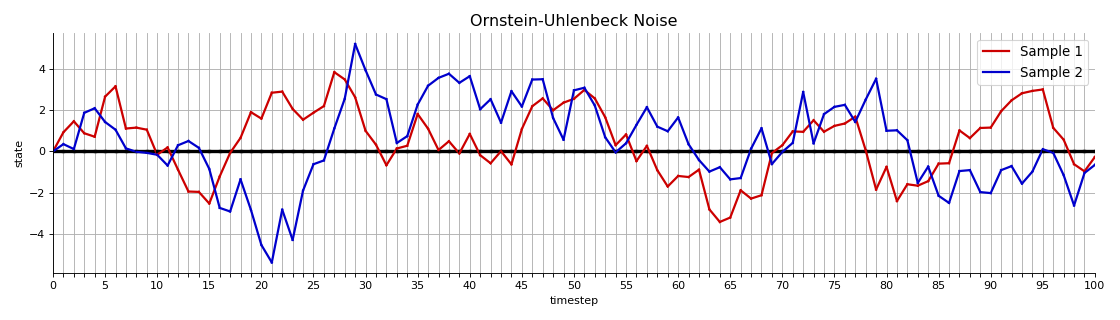
\includegraphics[width=\textwidth]{Images/ornstein_uhlenbeck_noise.png}
\end{center}
\end{example}

\subsection{Deep Deterministic Policy Gradient (DDPG)}

Мы собрали алгоритм DDPG --- off-policy алгоритм для непрерывных пространств действий. Несмотря на название, по свойствам этот алгоритм похож именно на DQN, и обладает аналогичными недостатками и преимуществами.

\begin{algorithm}[label = DDPGalgorithm]{Deep Deterministic Policy Gradient (DDPG)}
\textbf{Гиперпараметры:} $B$ --- размер мини-батчей, $\beta$ --- коэф. экспоненциального сглаживания для таргет-сеток, $\alpha, \sigma$ --- параметры шума, $Q_{\theta}(s, a)$ --- нейросетка с параметрами $\theta$, $\pi_{\omega}(s)$ --- детерминированная стратегия с параметрами $\omega$, SGD-оптимизаторы.

\vspace{0.3cm}
Инициализировать $\theta, \omega$ произвольно \\
Положить $\theta^- \coloneqq \theta$ \\
Положить $\omega^- \coloneqq \omega$ \\
Инициализировать шум $\eps \coloneqq 0$ \\
Пронаблюдать $s_0$ \\
\textbf{На очередном шаге $t$:}
\begin{enumerate}
    \item обновить шум $\eps \leftarrow \alpha \eps + \hat{\eps}$, где $\hat{\eps} \sim \N(0, \sigma^2 I)$
    \item выбрать $a_t \coloneqq \pi_\omega(s_t) + \eps$
    \item пронаблюдать $r_t$,  $s_{t+1}$, $\done_{t+1}$
    \item добавить пятёрку $(s_t, a_t, r_t, s_{t+1}, \done_{t+1})$ в реплей буфер
    \item засэмплировать мини-батч размера $B$ из буфера
    \item сделать один шаг градиентного подъёма по $\omega$:
    $$\frac{1}{B}\sum_{s \in B} Q_{\theta}(s, \pi_\omega(s)) \to \max_{\omega}$$
    \item для каждого перехода $\T \coloneqq (s, a, r, s', \done)$ посчитать таргет:
    $$y(\T ) \coloneqq r + \gamma (1 - \done) Q_{\theta^{-}} \left( s', \pi_{\omega^{-}} \left( s' \right) \right)$$
    \item сделать один шаг градиентного спуска по $\theta$:
    $$\frac{1}{B}\sum_{\T} \left( Q_{\theta}(s, a) - y(\T ) \right) ^2 \to \min_\theta$$
    \item если $t \operatorname{mod} K = 0$: 
        $$\theta^{-} \gets (1 - \beta) \theta^{-} + \beta \theta$$
        $$\omega^{-} \gets (1 - \beta) \omega^{-} + \beta \omega$$
\end{enumerate}
\end{algorithm}

\begin{remark}
DDPG за счёт off-policy режима может оказаться эффективнее PPO в задаче локомоции \ref{ex:locomotion}. В этой задаче нет тех проблем, из-за которых off-policy обучение может сломаться или плохо работать: там нет сильно отложенного сигнала (плохое действие --- и существо сразу падает, хорошее действие --- и существо продвинется вперёд и получит положительное подкрепление), Q-функция как функция от действий не похожа на плато (интуитивно, в большинстве состояний есть <<хорошие>> действия с высоким значением $Q(s, a)$, которые позволяют существу продолжать бежать, и <<плохие>> с низким значением, которые нарушают баланс устойчивости существа и приводят к его падению), а функция награды очень плотная и информативная, из-за чего полезно иметь возможность все переходы много раз из буфера вспоминать и обучаться восстанавливать хотя бы $r(s, a)$, содержащуюся в одношаговых таргетах, из разных пар $s, a$.
\end{remark}

\subsection{Twin Delayed DDPG (TD3)}\label{subsec:td3}

TD3 --- набор из трёх эвристических костылей, которые можно навесить над DDPG для существенного повышения стабильности происходящих процессов.

Одна из главных проблем DDPG --- унаследованная от DQN проблема переоценивания (см. раздел \ref{subsec:overestimation}). Хотя сейчас в формулах в явном виде не присутствует оператор максимума, на самом деле он всё равно есть: наш актёр учится <<взламывать>> критика и находить те действия, где погрешность нашей аппроксимации истинной Q-функции положительна. Поэтому оценка $Q_\theta (s, \pi_\omega(s))$ практически всегда завышенно оценивает $\max\limits_a Q^\pi(s, a)$, и если это завышение попадает в целевую переменную для обучения модели Q-функции, начинается цепная реакция. 

\needspace{7\baselineskip}
\begin{wrapfigure}[9]{r}{0.35\textwidth}
%\vspace{-0.5cm}
\centering
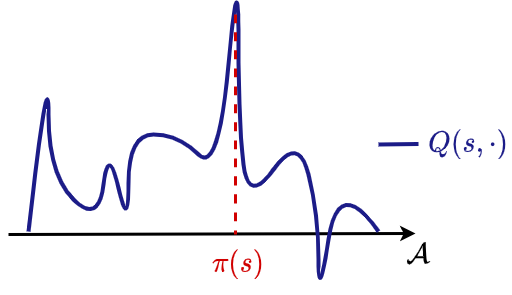
\includegraphics[width=0.35\textwidth]{Images/TD3_overestimation.png}
%\vspace{-0.9cm}
\end{wrapfigure}

Более того, в пространстве действий могут обнаружиться узкие области, в которых наша неидеальная нейросетевая аппроксимация Q-функции имеет всплеск; актёр может научиться <<взламывать>> критика, используя эти всплески. Поэтому первая идея борьбы с этим эффектом заключается в том, чтобы при построении таргета зашумить выход нашей стратегии при помощи некоторого шума. Шум здесь не должен быть очень большим по модулю (важно, что этот шум не имеет смысл <<исследований>>): обычно сэмплируют зашумление из гауссианы и обрезают, чтобы получить что-то не очень большое по значению:
$$\eps' \sim \clip(\N(0, \hat{\sigma}I), -c, c)$$

Во-вторых, воспользуемся Twin-трюком, который мы обсуждали в разделе \ref{subsec:clippedtwin}, а то есть будем обучать две Q-функции по общему буферу и использовать в таргетах минимум из двух оценок критиков. Таргет-сеть обычно заводят для каждой из двух копий; а вот стратегию предлагается оставить для них общую, то есть использовать одно и то же <<приближение аргмакса>> для обоих Q-функций, поскольку в такой схеме она моделируется отдельной нейросетью. Итого формула таргета получается общая для двух критиков:
$$y(\T ) \coloneqq r + \gamma \min_{i \in \{1, 2\}}Q_{\theta_i^{-}}( s', \pi_{\omega^{-}}(s') + \eps')$$

При обучении актёра можно как оставить оптимизацию при помощи первого из двух критиков
$$Q_{\theta_1}(s, \pi_\omega(s)) \to \max_{\omega},$$
и тогда актёр не будет видеть одну из Q-функций (и там, где у первого критика будет взломанное актёром завышение, у второго критика, мы надеемся, завышение или занижение будет условно равновероятно), так и использовать снова минимум из двух критиков:
$$\min_{i \in \{1, 2\}} Q_{\theta_i}(s, \pi_\omega(s)) \to \max_{\omega}$$

Наконец, в-третьих, обновление весов стратегии будем делать реже, чем обновление весов Q-функции: это позволит <<поучить>> Q-функцию приближать $Q^\pi$ именно для текущей, свежей версии $\pi$, прежде чем использовать её градиент для оптимизации стратегии; здесь наблюдается полная аналогия с GAN-ами, где тоже иногда помогают подобные фокусы.

\begin{remark}
Третья эвристика кажется наименее существенной, поскольку авторы предлагали делать $N \HM= 2$ шагов обучения критика на один шаг обучения актёра.
\end{remark}

\begin{algorithm}[label = TD3]{Twin Delayed DDPG (TD3)}
\textbf{Гиперпараметры:} $B$ --- размер мини-батчей, $N$ --- периодичность обновления весов стратегии, $\alpha, \sigma$ --- параметры шума, $\hat{\sigma}, c$ --- параметры шума для добавки к действиям для таргета, $\beta$ --- коэф. экспоненциального сглаживания для таргет-сеток, $Q_{\theta_1}(s, a), Q_{\theta_2}(s, a)$ --- нейросетки с параметрами $\theta_1, \theta_2$, $\pi_{\omega}(s)$ --- детерминированная стратегия с параметрами $\omega$, SGD-оптимизаторы.

\vspace{0.3cm}
Инициализировать $\theta_1, \theta_2, \omega$ произвольно \\
Инициализировать таргет-сетки $\theta_1^- \coloneqq \theta_1, \theta_2^- \coloneqq \theta_2, \omega^- \coloneqq \omega$ \\
Инициализировать шум $\eps_0 \coloneqq 0$ \\
Пронаблюдать $s_0$ \\
\textbf{На очередном шаге $t$:}
\begin{enumerate}
    \item посчитать шум $\eps_{t} \coloneqq \alpha \eps_{t-1} + \eps$, где $\eps \sim \N(0, \sigma^2 I)$
    \item выбрать $a_t \coloneqq \pi_\omega(s_t) + \eps_{t}$
    \item пронаблюдать $r_t$,  $s_{t+1}$, $\done_{t+1}$
    \item добавить пятёрку $(s_t, a_t, r_t, s_{t+1}, \done_{t+1})$ в реплей буфер
    \item засэмплировать мини-батч размера $B$ из буфера
    \item для каждого перехода $\T \coloneqq (s, a, r, s', \done)$ посчитать таргет:
    $$\eps' \sim \clip(\N(0, \hat{\sigma}I), -c, c)$$
    $$y(\T ) \coloneqq r + \gamma (1 - \done) \min_{i \in \{1, 2\}}Q_{\theta_i^{-}}(s', \pi_{\omega^{-}}(s') + \eps')$$
    \item сделать один шаг градиентного спуска по $\theta_1$ и $\theta_2$:
    $$\frac{1}{B}\sum_{\T} \left( Q_{\theta_1}(s, a) - y(\T ) \right) ^2 \to \min_{\theta_1}$$
    $$\frac{1}{B}\sum_{\T} \left( Q_{\theta_2}(s, a) - y(\T ) \right) ^2 \to \min_{\theta_2}$$
    \item \textbf{если $t \operatorname{mod} N = 0$}:
    \begin{itemize}
        \item сделать один шаг градиентного подъёма по $\omega$:
        $$\frac{1}{B}\sum_{s \in B} Q_{\theta_1}(s, \pi_\omega(s)) \to \max_{\omega}$$
        \item обновить таргет-сети:
        $$\theta^{-}_1 \gets (1 - \beta) \theta^{-}_1 + \beta \theta_1$$
        $$\theta^{-}_2 \gets (1 - \beta) \theta^{-}_2 + \beta \theta_2$$
        $$\omega^{-}   \gets (1 - \beta) \omega^{-}   + \beta \omega$$
    \end{itemize}
\end{enumerate}
\end{algorithm}

\subsection{Обучение стохастичных политик}\label{subsec:stochpolicies}

Среди преимуществ on-policy режима, которые мы потеряли в off-policy алгоритмах, мы упоминали возможность обучать стохастичные политики. Действительно, ряд наших проблем с нестабильностью в DDPG был связан с тем, что мы учим детерминированную стратегию: нужны костыли для решения проблемы exploration-а, актёр может <<взламывать>> нашу аппроксимацию критика и приводить к overestimation-у, и всё это приходится лечить очередной порцией эвристик. Когда же в on-policy подходе мы можем получить, если так можно сказать, <<естественный>> exploration за счёт обучения стохастичной стратегии. Обязательно ли в off-policy режиме учить именно детерминированную стратегию?

На самом деле нет. В теории есть возможность обучать и стохастического актёра, хотя точные формулы градиента будут немного отличаться в зависимости от выбранной параметризации политики. Итак, допустим мы моделируем актёра $\pi_\theta(a \HM\mid s)$ в классе стохастичных стратегий.

\begin{definition}
Скажем, что для параметризации $\pi_\theta(a \HM\mid s)$ применим \emph{репараметризационный трюк} (reparameterization trick), если сэмплирование $a \HM\sim \pi_\theta(a \mid s)$ эквивалентно сэмплированию шума из некоторого не зависящего от параметров распределения $\eps \HM\sim p(\eps)$ и его дальнейшего детерминированного преобразования $a \HM= f_{\theta}(s, \eps)$.
\end{definition}

\begin{exampleBox}[label=ex:gaussian_policy]{}
Пусть наша стратегия параметризована нормальным распределением:
$$\pi_\theta(a \HM\mid s) \HM\coloneqq \N(\mu_\theta(s), \sigma_\theta(s)^2I)$$
Тогда для неё применим репараметризационный трюк: сэмплирование действий эквивалентно $a \coloneqq \mu_\theta(s) \HM+ \eps \HM\odot \sigma_\theta(s)$, где $\eps \HM\sim \N(0, I)$, $\odot$ --- поэлементное перемножение.
\end{exampleBox}

\begin{example}
Семейство детерминированных стратегий $\pi_\theta(s)$ тоже можно считать таким <<вырожденным>> примером параметризаций, для которой можно проворачивать репараметризационный трюк: просто шум $\eps$ считаем <<пустым>>.
\end{example}

Можно заметить, что если для семейства стратегий применим репараметризационный трюк, то в выводе формулы Policy Gradient можно пользоваться им вместо REINFORCE: фактически, в теореме \ref{th:dpg} мы этим воспользовались.

\begin{theorem}
Если для $\pi_\theta(a \HM\mid s)$ применим репараметризационный трюк, то:
\begin{equation}\label{rt_dpg}
\nabla_\theta J(\pi_\theta) = \frac{1}{1 - \gamma}\E_{d_{\pi_\theta}(s)} \E_{\eps \HM\sim p(\eps)} \nabla_\theta f_\theta(s, \eps) \left. \nabla_a Q^{\pi}(s, a) \right|_{a = f_\theta(s, \eps)}
\end{equation}
\begin{proof}
Полностью полностью повторяет вывод теоремы \ref{th:dpg}.
\end{proof}
\end{theorem}

Таким образом, все идеи DDPG расширяются на этот случай. Убирая из формулы градиента частоты посещения состояний и переходя к policy iteration схеме, получаем следующий функционал:
\begin{equation}\label{general_pi_ddpg}
\E_s \E_{a \sim \pi_\theta(a \mid s)} Q_\omega(s, a) \to \max_{\theta},
\end{equation}
где состояния берутся из буфера. В силу репараметризационного трюка мы легко справимся со взятием градиента на практике:
\begin{equation*}
\nabla_\theta \E_{a \sim \pi_\theta(a \mid s)} Q_\omega(s, a) = \E_{\eps \sim p(\eps)} \nabla_\theta Q_\omega(s, f_{\theta}(s, \eps))
\end{equation*}
Теперь стохастическая оценка градиента по $\theta$ получается напрямую. Понятно, что мы получили обобщение формулы \eqref{ddpg_actor}; мы оптимизируем актёра при помощи градиентов из критика, но дополнительно впрыскиваем шум в действия для получения стохастичной стратегии. 

Недостатком гауссианы является то, что она унимодальна, что может приводить к бедам.

\begin{exampleBox}[righthand ratio=0.35, sidebyside, sidebyside align=center, lower separated=false]{}
Представьте, что вы хотите объехать дерево. Вы можете объехать его справа, можете слева. Критик сообщает вам высокие значения и слева, и справа, и оптимизируя \eqref{general_pi_ddpg} в классе гауссиан, можно получить стратегию, которая с наибольшей вероятностью выбирает действие <<врезаться в дерево>>.

\tcblower
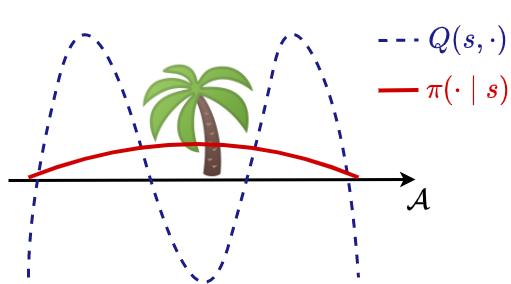
\includegraphics[width=\textwidth]{Images/Multimodal1.png}
\end{exampleBox}

Поэтому мы можем захотеть выбрать более сложную параметризацию стратегии, для которой не применим репараметризационный трюк.

\begin{exampleBox}[label=ex:gaussianmixture_policy, righthand ratio=0.35, sidebyside, sidebyside align=center, lower separated=false]{}
Например, можно использовать смесь гауссиан. Тогда при использовании $K$ компонент смеси актёр для данного состояния $s$ выдаёт следующие величины: $K$ суммирующихся в единицу чисел $w_i(s, \theta)$, а также $K$ векторов $\mu_i(s, \theta), \sigma_i(s, \theta)$, где $i \in {1, 2, \dots, K}$. Итоговое распределение полагается
$$\pi_\theta(a \mid s) \coloneqq \sum_{i = 1}^K w_i(s, \theta) \N(\mu_i(s, \theta), \sigma_i(s, \theta)^2I)$$

\tcblower
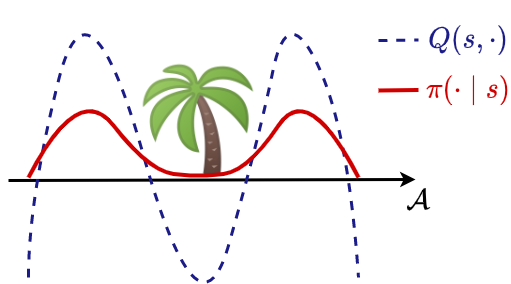
\includegraphics[width=\textwidth]{Images/Multimodal2.png}
\end{exampleBox}

Тогда для оптимизации \eqref{general_pi_ddpg} нам придётся использовать REINFORCE, обладающий более высокой дисперсией оценок, для сбивания которой необходимо использование бэйзлайна:

\begin{proposition}
Градиент \eqref{general_pi_ddpg} по параметрам актёра $\theta$ равен
$$\nabla_\theta = \E_{a \sim \pi_\theta(a \mid s)} \nabla_{\theta} \log \pi_\theta(a \mid s) \left( Q_\omega(s, a)(s, a) - b(s) \right),$$
где $b(s)$ --- бэйзлайн, произвольная функция от состояний.
\end{proposition}

Естественно, эту формулу можно интерпретировать как то, что в обычной формуле policy gradient \eqref{pgt_baseline} мы аналогично DDPG <<отказались>> от сэмплирования состояний из частот посещения текущей стратегии ради off-policy режима работы. Ну и хорошим бэйзлайном будет, соответственно, $V_\omega(s) \coloneqq \E_{a \sim \pi_\theta(a \mid s)} Q_\omega(s, a)$. Чтобы посчитать такое значение, можно либо использовать Монте-Карло оценку, либо учить отдельную нейросеть, аппроксимирующую V-функцию (целевой переменной для входа $s$ тогда будет $Q_\omega(s, a)$, где $a \HM\sim \pi_\theta(a \HM\mid s)$).

Обсудим ещё одну тонкость. В задачах непрерывного управления мы обычно работаем с пространством действий $|\A| \subseteq [-1, 1]^A$, и хотелось бы, чтобы наши семейства стратегий тоже выдавали действия именно из этого диапазона. Когда мы работали с детерминированными стратегиями, можно было учесть это в параметризации простым навешиванием гиперболического тангенса $\tanh$ на последний слой сети. А что, если мы используем гауссиану или смесь гауссиан?

\begin{remark}
Как ни странно, игнорирование этого нюанса может всё равно сработать на практике. То есть, актёр моделирует гауссиану, и считает, что он отправил сэмплы $a$ в среду, которые могут выходить за требуемый диапазон. Неожиданное преимущество такого подхода в том, что иногда в задачах <<оптимальные>> действия находятся на границе и равны +1 или -1 в каких-то компонентах, и тогда такая необрезанная гауссиана может довольно удобно <<часто>> сэмплировать подобные действия. Тем не менее, чаще имеет смысл всё же учесть домен в параметризации. 
\end{remark}

Тогда можно применять гиперболический тангенс к сэмплам из <<необрезанной>> модели. То есть, стратегия объявляется следующей: $\pi_\theta(a \HM \mid s) \coloneqq \tanh(u)$, где $u \HM \sim \mu_\theta(u \HM \mid s)$, и $u \HM \in \R^A$. Понятно, как тогда применять репараметризационный трюк, но если мы пользуемся этой идеей вместе с REINFORCE (например, для обучения смеси гауссиан или в on-policy алгоритмах), то нам нужно уметь считать $\log \pi_\theta(a \HM \mid s)$. Для этого нужно вспоминать правило замены переменных в плотностях (см., например, \href{https://ru.wikipedia.org/wiki/Плотность_вероятности#Плотность_преобразования_случайной_величины}{википедию}).

\begin{theorem}[Формула замены переменной в плотности]
Пусть $\pi_\theta(a \HM \mid s) \coloneqq g(u)$, где $g \colon \R^A \to \R^A$, и $u \HM \sim \mu_\theta(u \HM \mid s)$. Тогда:

\begin{equation}\label{changeofvariabledensity}
\log \pi_\theta(a \HM \mid s) = \log \mu_\theta(a \HM \mid s) - \log | \det \nabla_u g | 
\end{equation}
\end{theorem}

\begin{example}
Например, для функции $g(u) \coloneqq \tanh (u)$ якобиан $\nabla_u g$ есть диагональная матрица (поскольку преобразование поэлементное), и его определитель равен покомпонентному произведению:
\begin{align*}
\det \nabla_u g(u) &= \prod_{i=1}^{A} \nabla_{u_i} \tanh(u_i) = \\
= \{ \text{производная гиперболического тангенса} \} &= \prod_{i=1}^A (1 - \tanh^2(u_i))    
\end{align*}
Заметим, что все компоненты положительные ($\tanh(u_i) \HM \le 1$), поэтому модуль из формулы \eqref{changeofvariabledensity} брать не нужно. Подставляя в \eqref{changeofvariabledensity}, получаем окончательно:
$$\log \pi_\theta(a \HM \mid s) = \log \mu_\theta(a \HM \mid s) - \sum_{i=1}^A \log (1 - \tanh^2(u_i)) $$
\end{example}

Итак, теоретически возможность обучать стохастичные стратегии в off-policy режиме есть. Что тогда мешает в DDPG воспользоваться этим и использовать гауссиану или смесь гауссиан? Дело в том, что мы помним, что направление оптимизации актёра --- детерминированная стратегия: мы идём в сторону жадной стратегии $\pi_\theta(s) \HM= \argmax\limits_a Q_\omega(s, a)$. Схлопывание стохастичной стратегии в детерминированную чревато численными проблемами: например, для гауссианы дисперсия начнёт уходить в ноль, градиенты могут начать взрываться.

Можно, конечно, попытаться как-то побороться с этим эффектом, например, при помощи эвристики, которой часто пользуются в on-policy методах --- добавкой энтропийного лосса. Напомним: чем больше значение энтропии для распределения, тем оно <<менее вырожденное>>:

\begin{definition}
Энтропией распределения $\pi(a)$ называется
\begin{equation}\label{entropydef}
\entropy(\pi(a)) \coloneqq - \E_{\pi(a)} \log \pi(a)
\end{equation}
\end{definition}

И в policy gradient алгоритмах часто в формулу градиента добавляют слагаемое $\nabla_{\theta} \entropy(\pi_\theta(\cdot \mid s))$, которое поощряет высокую энтропию стратегии. Однако в on-policy режиме Q-функция заменялась на оценку и была стохастичной. В off-policy же актёр имеет куда больше шансов <<переобучиться>> под критика, и энтропийный лосс придётся тогда выставлять с большим коэффициентом.

Вместо подобных плясок с бубном хотелось бы, чтобы подобных проблем в принципе не возникало. Конечно, детерминированность оптимальной стратегии --- особенность постановки задачи RL, и поэтому если мы хотим, чтобы таких эффектов в оптимизационных процессах не было, нам придётся найти какую-то альтернативную постановку задачи. Оказывается, такая альтернативная формулировка есть, и она бывает крайне удобна. В ней оптимальные стратегии уже будут стохастичны, и ряд численных проблем, а также проблем с exploration-ом, отпадёт; в частности, она <<обоснует>> добавку градиента энтропии в формулу градиента.